% Author: Izaak Neutelings (September 2020)
\documentclass[border=3pt,tikz]{standalone}
\usepackage{physics}
\usepackage{tikz}
\usetikzlibrary{patterns,snakes}

\colorlet{xcol}{blue!70!black}
\colorlet{myred}{red!65!black}
\tikzstyle{ground}=[preaction={fill,top color=black!10,bottom color=black!5,shading angle=20},
                    fill,pattern=north east lines,draw=none,minimum width=0.3,minimum height=0.6]
\tikzstyle{mass}=[line width=0.6,red!30!black,fill=red!40!black!10,rounded corners=1,
                  top color=red!40!black!20,bottom color=red!40!black!10,shading angle=20]
\tikzstyle{spring}=[line width=0.8,black!80,snake=coil,segment amplitude=5,segment length=5,line cap=round]
\tikzset{>=latex} % for LaTeX arrow head
\def\tick#1#2{\draw[thick] (#1) ++ (#2:0.1) --++ (#2-180:0.2)} %0.03*\xmax
\tikzstyle{force}=[->,myred,very thick,line cap=round]
\def\tick#1#2{\draw[thick] (#1)++(#2:0.12) --++ (#2-180:0.24)}

\begin{document}


% HORIZONTAL ground
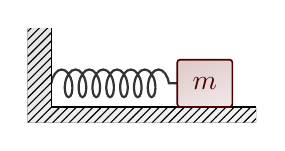
\begin{tikzpicture}
  \def\H{1}   % wall height
  \def\T{0.3} % wall thickness
  \def\L{2.6} % ground length
  \def\D{0.2} % ground depth
  \def\h{0.6} % mass height
  \def\w{0.7} % mass width
  \def\x{1.6} % mass x position
  \draw[spring] (0,\h/2) --++ (\x,0);
  \draw[ground] (0,0) |-++ (-\T,\H) |-++ (\T+\L,-\H-\D) -- (\L,0) -- cycle;
  \draw (0,\H) -- (0,0) -- (\L,0);
  \draw[mass] (\x,0) rectangle++ (\w,\h) node[midway] {$m$};
\end{tikzpicture}


% HORIZONTAL ground - axis
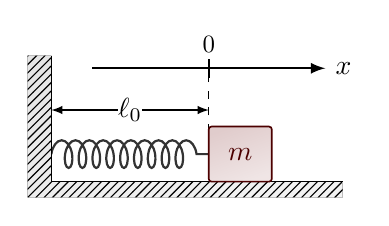
\begin{tikzpicture}
  \def\H{1.6} % wall height
  \def\T{0.3} % wall thickness
  \def\L{3.7} % ground length
  \def\D{0.2} % ground depth
  \def\h{0.7} % mass height
  \def\w{0.8} % mass width
  \def\x{2.0} % mass x position
  \def\y{0.9*\H} % x axis y position
  \draw[->,thick] (\x-0.4*\L,\y) -- (\x+0.4*\L,\y) node[right] {$x$};
  \tick{\x,\y}{-90} node[scale=0.9,above=-1] {$0$};
  \draw[<->] (0,1.3*\h) --++ (\x,0) node[midway,fill=white,inner sep=0] {$\ell_0$};
  \draw[spring] (0,\h/2) --++ (\x,0);
  \draw[ground] (0,0) |-++ (-\T,\H) |-++ (\T+\L,-\H-\D) -- (\L,0) -- cycle;
  \draw[dashed] (\x,0.9*\h) --++ (0,\y-0.9*\h);
  \draw (0,\H) -- (0,0) -- (\L,0);
  \draw[mass] (\x,0) rectangle++ (\w,\h) node[midway] {$m$};
\end{tikzpicture}


% HORIZONTAL ground - axis, extended
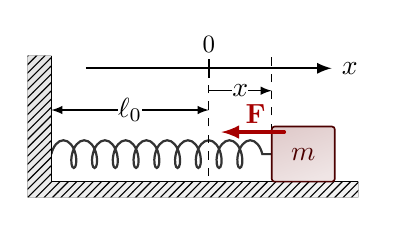
\begin{tikzpicture}
  \def\H{1.6} % wall height
  \def\T{0.3} % wall thickness
  \def\L{3.9} % ground length
  \def\D{0.2} % ground depth
  \def\h{0.7} % mass height
  \def\w{0.8} % mass width
  \def\x{2.0} % mass x position
  \def\dx{0.8} % extension
  \def\y{0.9*\H} % x axis y position
  \def\F{0.8} % force
  \draw[->,thick] (\x-0.4*\L,\y) -- (\x+0.4*\L,\y) node[right] {$x$};
  \tick{\x,\y}{-90} node[scale=0.9,above=-1] {$0$};
  \draw[<->] (0,1.3*\h) --++ (\x,0) node[midway,fill=white,inner sep=0] {$\ell_0$};
  \draw[->] (\x,1.65*\h) --++ (\dx,0) node[midway,fill=white,inner sep=0] {$x$};
  \draw[spring,segment length=7.5] (0,\h/2) --++ (\x+\dx,0);
  \draw[ground] (0,0) |-++ (-\T,\H) |-++ (\T+\L,-\H-\D) -- (\L,0) -- cycle;
  \draw (0,\H) -- (0,0) -- (\L,0);
  \draw[dashed]
    (\x,0.1*\h) --++ (0,\y-0.1*\h)
    (\x+\dx,0.9*\h) --++ (0,1.1*\y-0.9*\h);
  \draw[mass] (\x+\dx,0) rectangle++ (\w,\h) node[midway] {$m$};
  \draw[force] (\x+\dx+0.2*\w,0.9*\h) --++ (-\F,0) node[midway,right=1,above=-1] {$\vb{F}$};
\end{tikzpicture}


% HORIZONTAL ground - axis, compressed
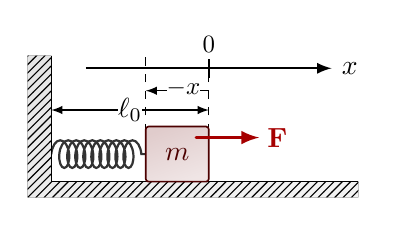
\begin{tikzpicture}
  \def\H{1.6} % wall height
  \def\T{0.3} % wall thickness
  \def\L{3.9} % ground length
  \def\D{0.2} % ground depth
  \def\h{0.7} % mass height
  \def\w{0.8} % mass width
  \def\x{2.0} % mass x position
  \def\dx{0.8} % extension
  \def\y{0.9*\H} % x axis y position
  \def\F{0.8} % force
  \draw[->,thick] (\x-0.4*\L,\y) -- (\x+0.4*\L,\y) node[right] {$x$};
  \tick{\x,\y}{-90} node[scale=0.9,above=-1] {$0$};
  \draw[<->] (0,1.3*\h) --++ (\x,0) node[midway,fill=white,inner sep=0] {$\ell_0$};
  \draw[->] (\x,1.65*\h) --++ (-\dx,0) node[midway,above=1,right=-4,fill=white,inner sep=0,scale=0.9] {$-x$};
  \draw[spring,segment length=2.9] (0,\h/2) --++ (\x-\dx,0);
  \draw[ground] (0,0) |-++ (-\T,\H) |-++ (\T+\L,-\H-\D) -- (\L,0) -- cycle;
  \draw (0,\H) -- (0,0) -- (\L,0);
  \draw[dashed]
    (\x,0.9*\h) --++ (0,\y-0.9*\h)
    (\x-\dx,0.9*\h) --++ (0,1.1*\y-0.9*\h);
  \draw[mass] (\x-\dx,0) rectangle++ (\w,\h) node[midway] {$m$};
  \draw[force] (\x-\dx+0.8*\w,0.8*\h) --++ (\F,0) node[below=0,right=-1] {$\vb{F}$};
\end{tikzpicture}


% VERTICAL ceiling
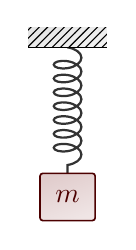
\begin{tikzpicture}
  \def\H{0.25} % ceiling height
  \def\W{1.0}  % ceiling width
  \def\h{0.6}  % mass height
  \def\w{0.7}  % mass width
  \def\y{1.6}  % mass width
  \draw[spring] (0,0) -- (0,-\y);
  \draw[ground] (-\W/2,0) rectangle++ (\W,\H);
  \draw (-\W/2,0) --++ (\W,0);
  \draw[mass] (-\w/2,-\y) rectangle++ (\w,-\h) node[midway] {$m$};
\end{tikzpicture}


% VERTICAL ceiling - no mass
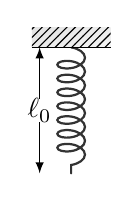
\begin{tikzpicture}
  \def\H{0.25} % ceiling height
  \def\W{1.0}  % ceiling width
  \def\h{0.6}  % mass height
  \def\w{0.7}  % mass width
  \def\y{1.6}  % mass width
  \draw[spring] (0,0) -- (0,-\y);
  \draw[ground] (-\W/2,0) rectangle++ (\W,\H);
  \draw (-\W/2,0) --++ (\W,0);
  \draw[<->] (-0.4*\W,0) --++ (0,-\y) node[midway,fill=white,inner sep=0] {$\ell_0$};
\end{tikzpicture}


% VERTICAL ceiling - elongation
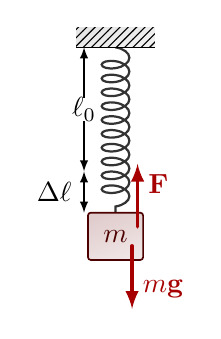
\begin{tikzpicture}
  \def\H{0.25} % ceiling height
  \def\W{1.0}  % ceiling width
  \def\h{0.6}  % mass height
  \def\w{0.7}  % mass width
  \def\y{2.1}  % mass width
  \def\F{0.8}  % force magnitude
  \draw[spring] (0,0) -- (0,-\y);
  \draw[ground] (-\W/2,0) rectangle++ (\W,\H);
  \draw (-\W/2,0) --++ (\W,0);
  \draw[mass] (-\w/2,-\y) rectangle++ (\w,-\h) node[midway] {$m$};
  \draw[force] (0.4*\w,-\y-0.3*\h) --++ (0,\F) node[below right=0] {$\vb{F}$};
  \draw[force] (0.3*\w,-\y-0.7*\h) --++ (0,-\F) node[above right=0] {$m\vb{g}$};
  \draw[<->] (-0.4*\W,0) --++ (0,-0.75*\y) node[midway,fill=white,inner sep=0] {$\ell_0$};
  \draw[<->] (-0.4*\W,-0.75*\y) --++ (0,-0.25*\y) node[midway,left=1] {$\Delta\ell$};
\end{tikzpicture}


% VERTICAL ceiling - elongation
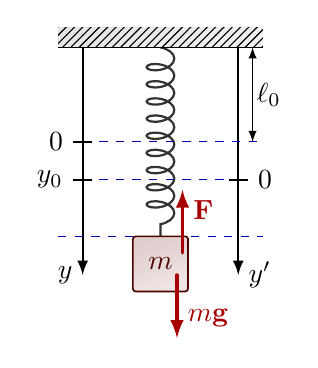
\begin{tikzpicture}
  \def\H{0.25}     % ceiling height
  \def\W{2.6}      % ceiling width
  \def\h{0.7}      % mass height
  \def\w{0.7}      % mass width
  \def\l{0.5*\y}   % rest length without weight
  \def\dl{0.7*\y}  % rest length with weight
  \def\y{2.4}      % mass y position
  \def\xy{0.38*\W} % mass y position
  \def\F{0.8}      % force magnitude
  \draw[spring,segment length=6.2] (0,0) -- (0,-\y);
  \draw[ground] (-\W/2,0) rectangle++ (\W,\H);
  \draw (-\W/2,0) --++ (\W,0);
  \draw[->,thick] (-\xy,0) --++ (0,-\y-0.7*\h) node[left] {$y$};
  \draw[->,thick] ( \xy,0) --++ (0,-\y-0.7*\h) node[right] {$y'$};
  \draw[dashed,xcol] (-\xy,-\l) --++ (2.3*\xy,0);
  \draw[dashed,xcol] (-\xy,-\dl) --++ (2*\xy,0);
  \draw[dashed,xcol] (-0.5*\W,-\y) --++ (\W,0);
  \tick{-\xy,-\l}{0} node[left] {$0$};
  \tick{-\xy,-\dl}{0} node[left] {$y_0$};
  \tick{ \xy,-\dl}{180} node[right] {$0$};
  \draw[mass] (-\w/2,-\y) rectangle++ (\w,-\h) node[midway] {$m$};
  \draw[force] (0.4*\w,-\y-0.3*\h) --++ (0,\F) node[below right=0] {$\vb{F}$};
  \draw[force] (0.3*\w,-\y-0.7*\h) --++ (0,-\F) node[above right=0] {$m\vb{g}$};
  \draw[<->] (0.45*\W,0) --++ (0,-\l) node[midway,right=-2] {$\ell_0$};
  %\draw[<->] (-0.4*\W,-0.75*\y) --++ (0,-0.25*\y) node[midway,left=1] {$y_0$};
\end{tikzpicture}


% HORIZONTAL double
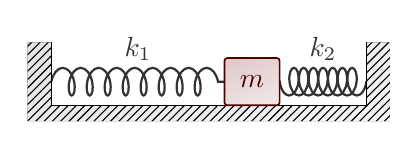
\begin{tikzpicture}
  \def\H{0.8} % wall height
  \def\T{0.3} % wall thickness
  \def\L{4.0} % ground length
  \def\D{0.2} % ground depth
  \def\h{0.6} % mass height
  \def\w{0.7} % mass width
  \def\x{2.2} % mass x position
  \draw[spring,segment length=6.5] (0,\h/2) --++ (\x,0) node[midway,above=4] {$k_1$};
  \draw[spring,segment length=3.5] (\L,\h/2) --++ (\x+\w-\L,0) node[midway,above=4] {$k_2$};
  \draw[ground] (0,0) |-++ (-\T,\H) |-++ (2*\T+\L,-\H-\D) |-++
                (-\T,\H+\D) --++ (0,-\H) -- cycle;
  \draw (0,\H) -- (0,0) -- (\L,0) --++ (0,\H);
  \draw[mass] (\x,0) rectangle++ (\w,\h) node[midway] {$m$};
  %\draw[force] (\x+0.1*\w,0.9*\h) --++ (-0.4*\L,0) node[midway,above=0] {$-k_1\vb{x}$};
  %\draw[force] (\x+0.9*\w,0.9*\h) --++ ( 0.2*\L,0) node[midway,above=0] {$-k_2\vb{x}$};
\end{tikzpicture}


\end{document}